\documentclass{IEEEtran}
\usepackage{graphicx}


\begin{document}

\title{Homework 5: Alpha-Beta, Dense Matrix Transform}
\author{Brandon Bell}
%\markboth{Brandon}{HW 2}
\maketitle
\begin{abstract}
\end{abstract}

\section{Large Messages Latency and Bandwidth}
$T(x) = T_S + T_C x $

\subsection{Comet}
 \begin{figure}
        \center{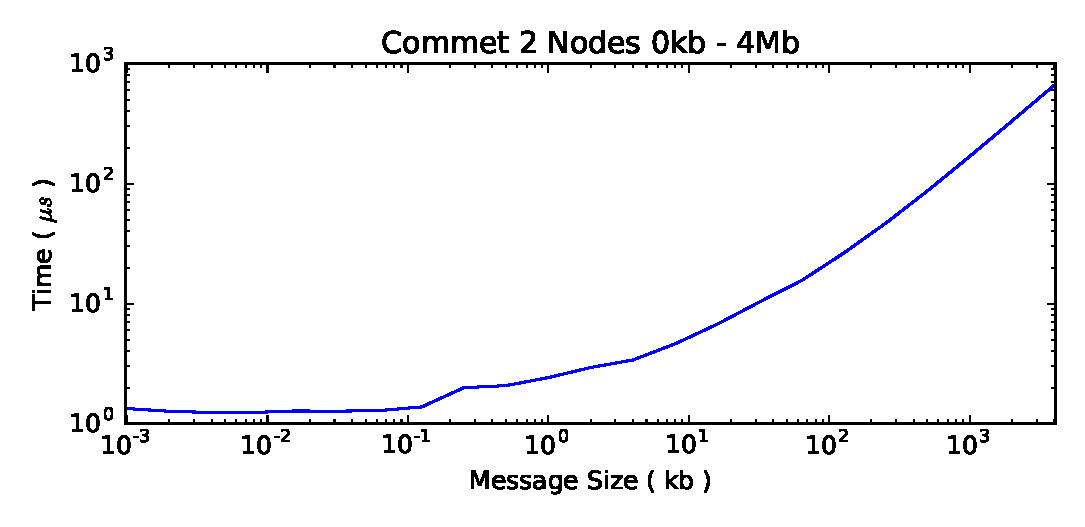
\includegraphics
        [width=8cm]{cld.eps}}
        \caption{ }
\end{figure}

 \begin{figure}
        \center{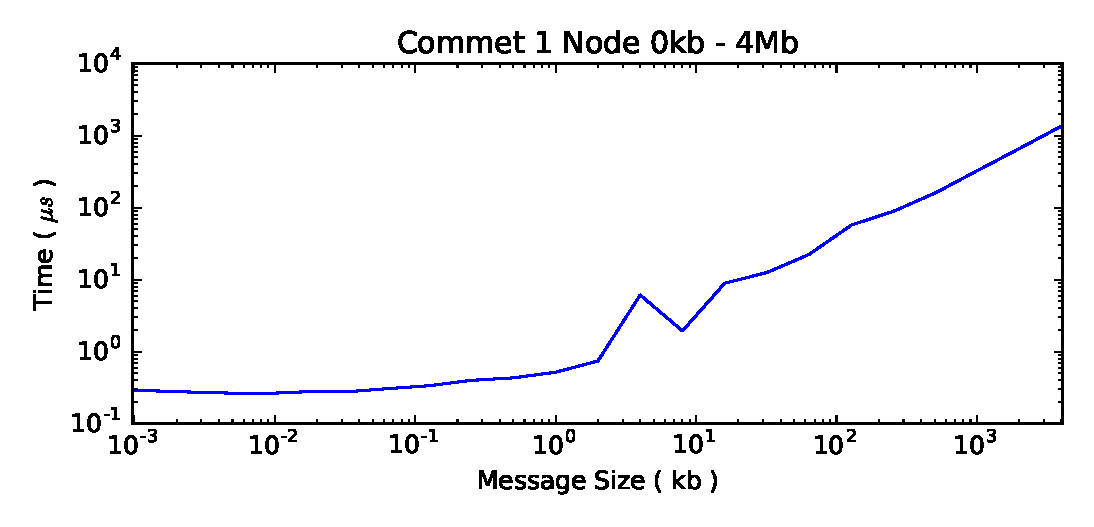
\includegraphics
        [width=8cm]{cls.eps}}
        \caption{ }
\end{figure}

 \begin{figure}
        \center{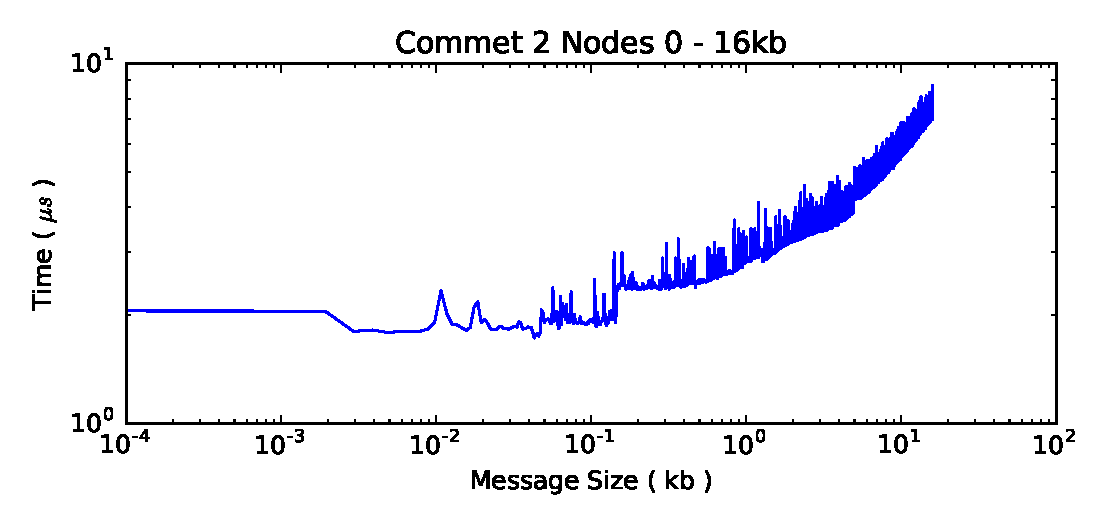
\includegraphics
        [width=8cm]{csd.eps}}
        \caption{ }
\end{figure}

\subsection{Stampede}
 \begin{figure}
        \center{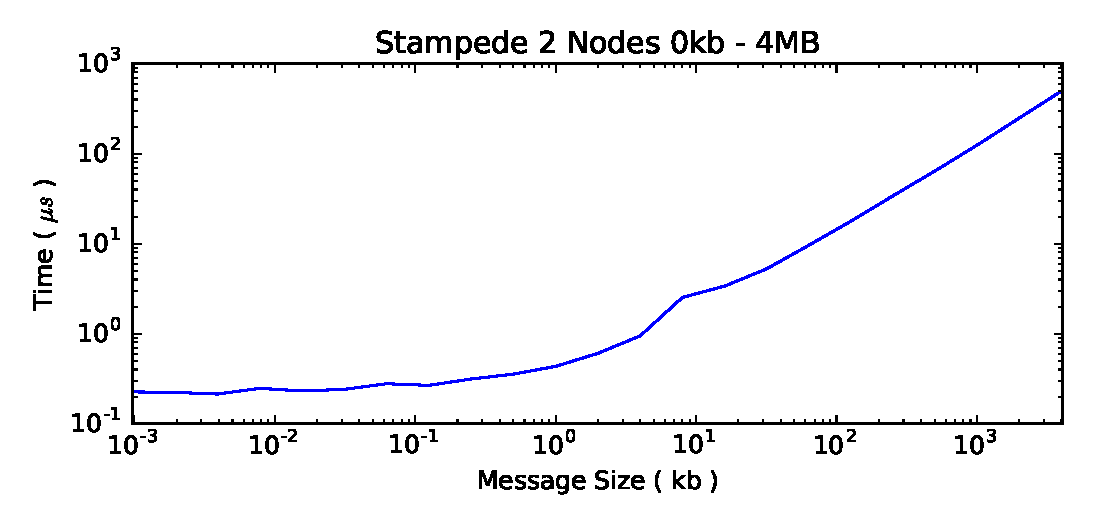
\includegraphics
        [width=8cm]{sls.eps}}
        \caption{ }
\end{figure}

 \begin{figure}
        \center{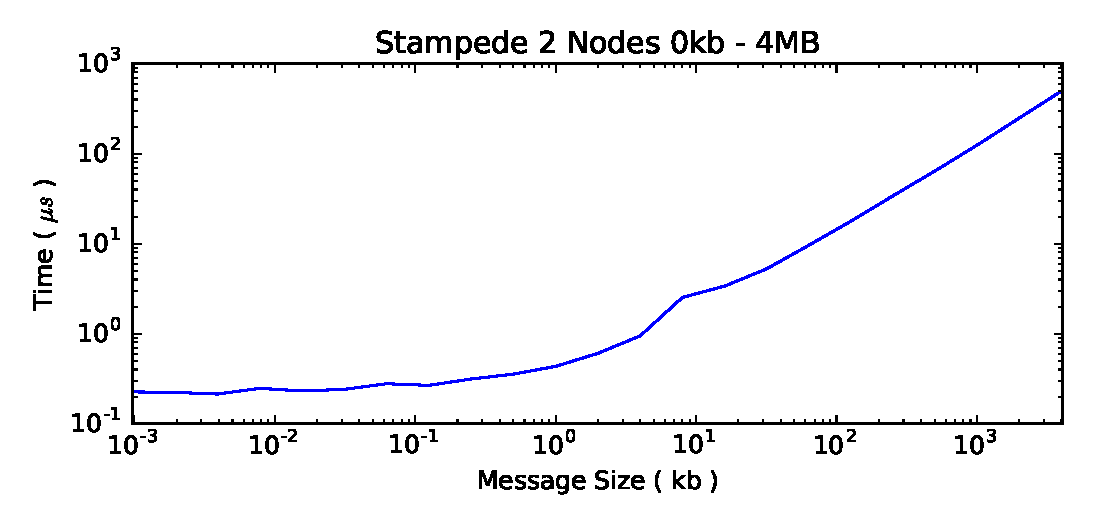
\includegraphics
        [width=8cm]{sls.eps}}
        \caption{ }
\end{figure}

 \begin{figure}
        \center{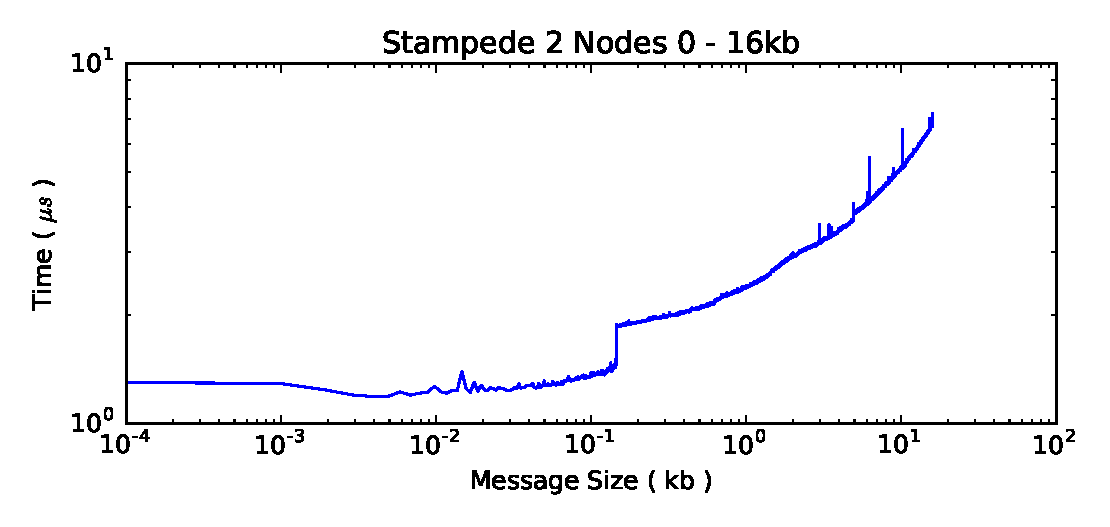
\includegraphics
        [width=8cm]{ssd.eps}}
        \caption{ }
\end{figure}




\end{document}
